\clearpage

\begin{center}
  {\color{accent}\large PART 2}\par
  \vspace{0.25em}
  {\Large\bfseries Chapter 2 應用：KNN Classification}\par
\end{center}

\vspace{1.0em}

\section*{1. Train/Test Split}
\sectionrule

這裡沿用 Part 1 整理出的 342 筆完整觀測，以及相同的四個 numerical features：culmen length、culmen depth、flipper length 與 body mass。要預測的 label 仍然是 species。

我使用 stratified train/test split，將 test size 設為 20\%，並固定 \dataterm{random\_state=42}。最後 training set 有 273 筆，test set 有 69 筆。採用分層抽樣，是希望三個物種在兩組資料中的比例都能接近原始分布。切分結果也已經依 \dataterm{source\_row} 保存，Part 4 的 Decision Tree 會直接沿用同一組 split。

\begin{table}[H]
\centering
\small
\begin{tabular}{lrrr}
\toprule
\textbf{Split} & \textbf{Adelie} & \textbf{Chinstrap} & \textbf{Gentoo} \\
\midrule
Training set & 121 & 54 & 98 \\
Test set & 30 & 14 & 25 \\
\bottomrule
\end{tabular}
\end{table}

\section*{2. KNN and Proximity Design}
\sectionrule

我用 Part 1 選出的四個 features 建立 KNN。三個設定都固定 $k=5$，並採用 majority vote（uniform weights），這樣就能把比較重點放在 proximity 與 preprocessing，而不會同時受到其他參數干擾。

對兩筆企鵝資料 $x$ 與 $z$，Euclidean distance 與 Manhattan distance 分別為
\[
d_2(x,z)=\sqrt{\sum_j(x_j-z_j)^2},
\qquad
d_1(x,z)=\sum_j\lvert x_j-z_j\rvert.
\]
Euclidean distance 可以理解成多維空間中的直線距離，對較大的座標差異也會比較敏感；Manhattan distance 則是把各 feature 的絕對差異加總起來。由於四個 features 都是 numerical attributes，兩種距離都能直接使用，也很適合拿來比較 proximity 設計的影響。

\section*{3. Preprocessing and Scaling Comparison}
\sectionrule

兩種 distance 都會受到 feature 尺度影響。資料中的 body mass 約為 2700--6300 g，數值範圍遠大於其他毫米欄位；如果直接計算 raw distance，體重很容易主導哪些企鵝會被視為鄰居。因此我把 scaling 前後的 KNN 放在一起比較。

Z-score standardization 使用
\[
z_j=\frac{x_j-\mu_j^{(train)}}{\sigma_j^{(train)}}.
\]
其中的平均數與標準差只用 training set 估計，再套用到 test set。程式以 \dataterm{Pipeline} 封裝 scaler 與 KNN，確保 preprocessing 的擬合過程不會先看到 test data。

我安排了以下三個設定：

\begin{enumerate}[leftmargin=1.7em,itemsep=0.35em]
  \item Raw Euclidean：保留原始單位，使用 Euclidean distance。
  \item Z-score Euclidean：先做 Z-score，再使用 Euclidean distance；與設定 1 隔離 scaling 的影響。
  \item Z-score Manhattan：維持相同 scaling，改用 Manhattan distance；與設定 2 隔離 proximity metric 的影響。
\end{enumerate}

\section*{4. Accuracy and Confusion Matrix}
\sectionrule

\begin{table}[H]
\centering
\small
\begin{tabularx}{\linewidth}{L{3.7cm}L{2.4cm}Yrr}
\toprule
\textbf{設定} & \textbf{Scaling} & \textbf{Proximity} & \textbf{正確筆數} & \textbf{Accuracy} \\
\midrule
Raw Euclidean & 無 & Euclidean ($p=2$) & 51 / 69 & 73.91\% \\
Z-score Euclidean & StandardScaler & Euclidean ($p=2$) & 69 / 69 & 100.00\% \\
Z-score Manhattan & StandardScaler & Manhattan ($p=1$) & 69 / 69 & 100.00\% \\
\bottomrule
\end{tabularx}
\end{table}

我選擇 Raw Euclidean 作為代表性設定。雖然它的 accuracy 最低，錯誤分布卻最能看出未處理尺度時，KNN 的 proximity 會受到什麼影響。其 error rate 為
\[
1-\text{accuracy}=1-\frac{51}{69}=\frac{18}{69}=26.09\%.
\]

\begin{figure}[H]
\centering
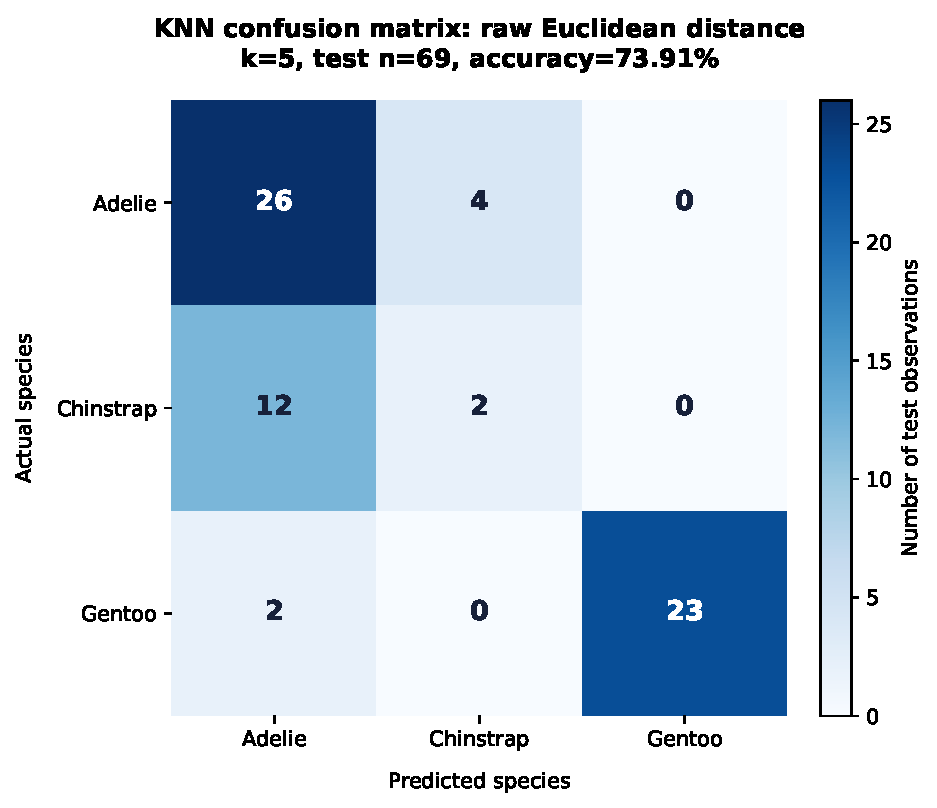
\includegraphics[width=0.62\linewidth]{part2_knn_confusion_matrix.pdf}
\caption{Raw Euclidean KNN 在 test set 的 confusion matrix。列為 actual class，欄為 predicted class。}
\end{figure}

\clearpage
\section*{5. Comparison and Discussion}
\sectionrule

從 confusion matrix 可以先看到，Raw Euclidean 對 14 筆 Chinstrap 只判對 2 筆，其中 12 筆被判成 Adelie；另外還有 4 筆 Adelie 被判成 Chinstrap。Gentoo 的辨識相對穩定，25 筆中判對 23 筆。這和尺度主導的預期一致：raw distance 大量受到 body mass 影響，喙部形態帶來的物種差異相對被壓低，所以 Adelie 與 Chinstrap 特別容易混淆。

做完 Z-score 後，四個 features 都改以各自的標準差為單位，Euclidean 設定在這組 test set 上將 69 筆全部判對。換句話說，scaling 確實改變了鄰居的組成，而且這個差異剛好修正了 raw distance 的 18 筆錯誤。StandardScaler 只用 training set 擬合，所以這項改善沒有使用 test label 或 test distribution 的資訊。

在相同的 Z-score preprocessing 下，Euclidean 與 Manhattan 得到完全相同的預測，accuracy 都是 100\%。對這組 split 來說，最明顯的差異來自 scaling；把 proximity 從 $L_2$ 改成 $L_1$，並沒有進一步改變分類結果。兩種 distance 當然不會永遠得到相同答案，這裡只能說，在目前的 features、$k=5$ 與固定 test set 下，它們選出的鄰居最後做出了相同的 majority vote。

這組比較最值得注意的地方，是資料尺度本身就會改變 KNN 所理解的「接近」。至於 100\% test accuracy，只能代表模型剛好把這 69 筆測試資料全部判對，不能直接推論它面對所有新資料都會完全正確。
